\documentclass[a4paper]{ctexart}
\usepackage[section]{placeins}
\usepackage{enumerate}
\usepackage[top=1in, bottom=1in, left=1.25in, right=1.25in]{geometry}
\usepackage{graphicx}
\usepackage{listings}

\author{\\\\\\\\\\\\\\\\REMOVED<REMOVED>\\学号:REMOVED\\班级: REMOVED\\REMOVED\\\\\\\\\\\\\\}
\title{微机原理实验5\\用STM32控制LCD1602}
\begin{document}

\begin{titlepage}
\maketitle
\thispagestyle{empty}
\newpage
\tableofcontents
\thispagestyle{empty}
\end{titlepage}

\setcounter{page}{1}
\lstset{language=C, 
    numbers=left, 
    frame=single,
    breaklines=true,
    breakautoindent=false,
    numberstyle=\tiny,
    fontadjust,
    basicstyle=\ttfamily
    }

\section{题目简介} 

将STM32链接到LCD1602上,并输出指定字符,或由串口输入的字符。

\section{题目分析}

LCD1602是一种液晶显示屏,大部分液晶显示屏使用的是HD44780U或者KS0066U之类的通用字库和
驱动芯片,这些芯片的驱动方法基本一样,因此通用性也比较强。下面介绍在测试过程中遇到的
几个问题和解决方法。

这个题目涉及到的技术细节有:
\begin{enumerate}[1.]
\item 和1602的对接方法
\item 实现比较精确的延迟
\item 1602操作方法
\end{enumerate}
下面对这几个要点分别进行说明

\subsection{和1602进行对接}

1602是5V器件,外接管脚主要有以下几类:
\begin{enumerate}
\item 供电管脚。主要有模块控制器5V供电、背景灯5V供电、对比度负电源VO(该电源一般从VC
C和GND之间用电阻分压取电)
\item 控制管脚。一般为三根线,分别为使能线E、读写控制线RW和指令/数据选择线RS
\item 数据管脚。D0~D7(使用4位控制则是D0~D3)
\end{enumerate}

供电管脚情况特殊,这里不对电气特性做讨论。控制管脚和数据管脚都是接入芯片控制端的,其
电气特性如下图\ref{elec1602}所示。
\begin{figure}[h]
  \centering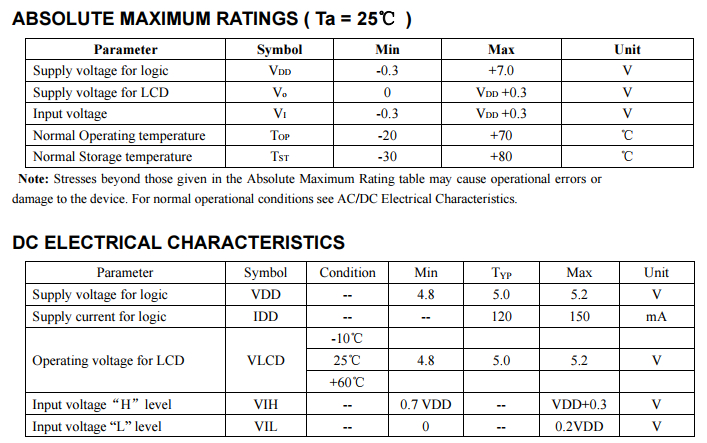
\includegraphics[width=\textwidth]{./img/1602_elec.png}
  \caption{Electrical Characteristics of LCD1602 Pins}\label{elec1602}
\end{figure}

可以看到,其中逻辑高低电平的最值分别是0.7倍的供电电平,也就是3.5V和0V,这样即使是作为
STM32的3.3V器件,也基本能轻松驱动这款芯片了。再结合下图\ref{stm32iodriver}中的驱动电
路图,所以对控制管脚使用推挽输出方法驱动芯片。如果这种驱动方法发生问题,那可以将管脚用
3.7k电阻上拉之后用晶体管控制电平值。
\begin{figure}[h]
  \centering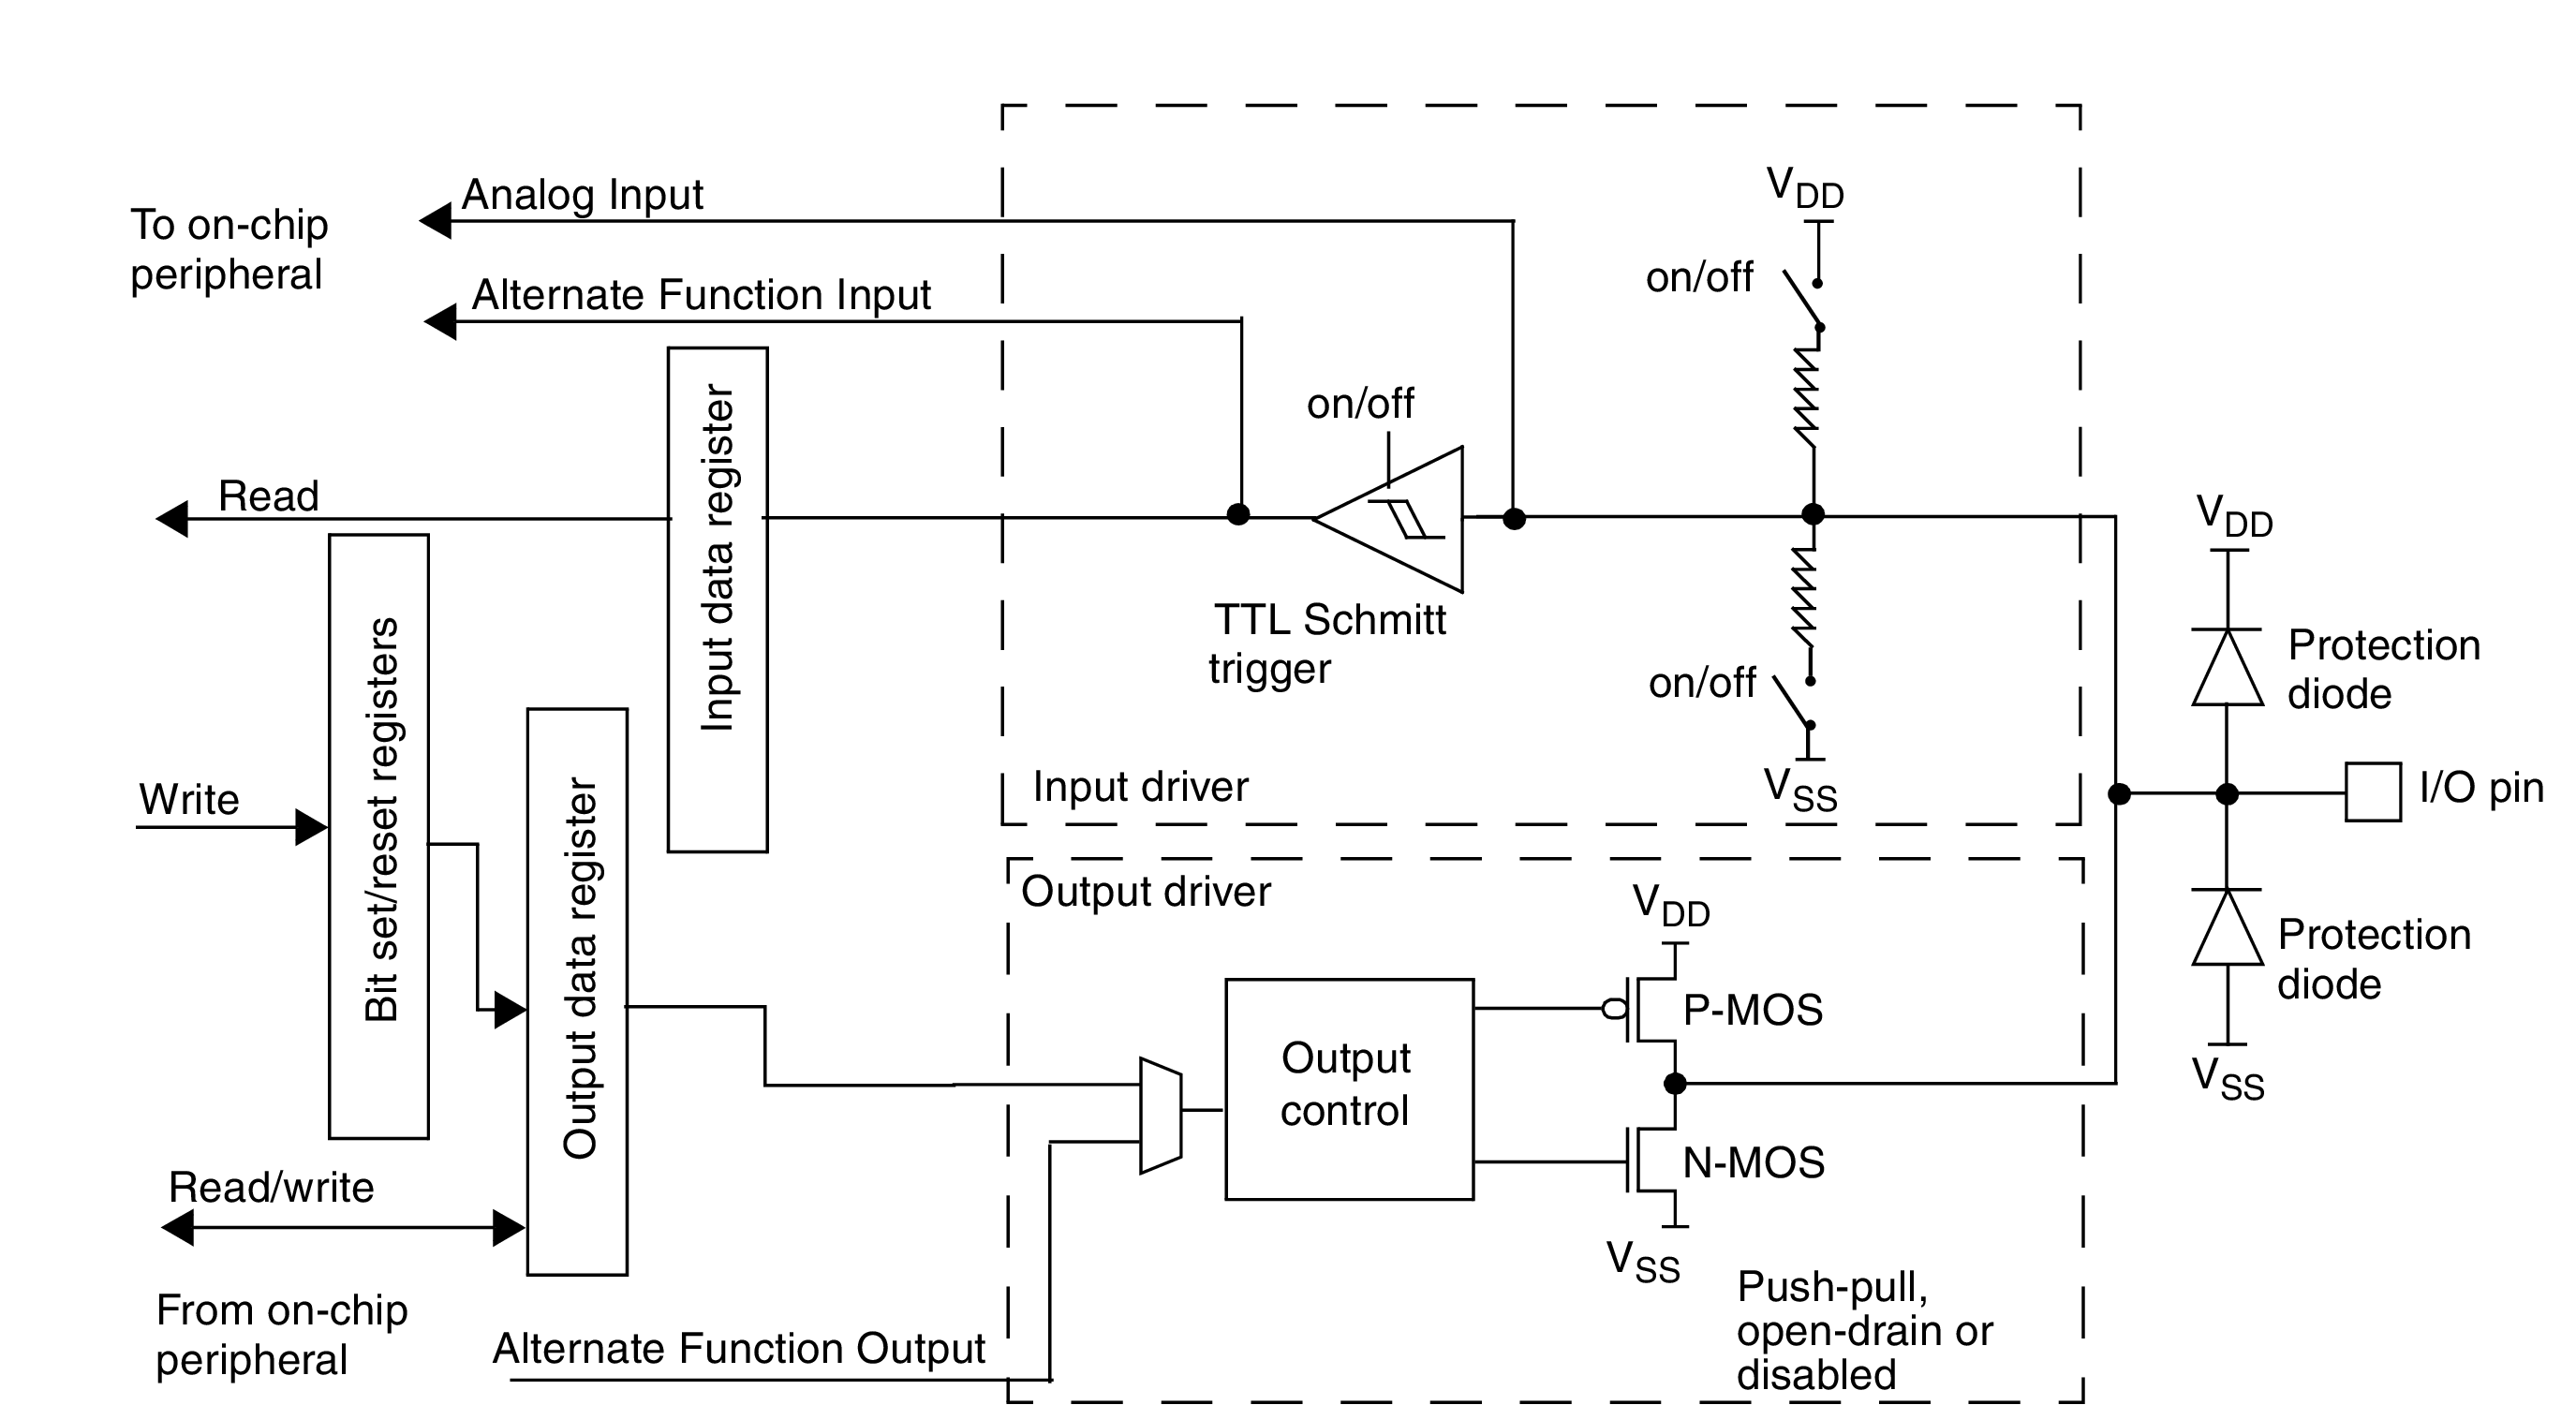
\includegraphics[width=\textwidth]{./img/ioport.png}
  \caption{STM32 IO Driver System}\label{stm32iodriver}
\end{figure}

相对于电气特性,另一个比较值得注意的就是读写时序问题。MCU的指令周期一般比较短(ns级
别),但控制器的响应时间比较久,因此要严格按照控制器的时序图进行读写。这一系列时序图
可以直接在Datasheet中找到,这里以写操作的时序图为例,如下图\ref{timing1602}:
\begin{figure}[h]
  \centering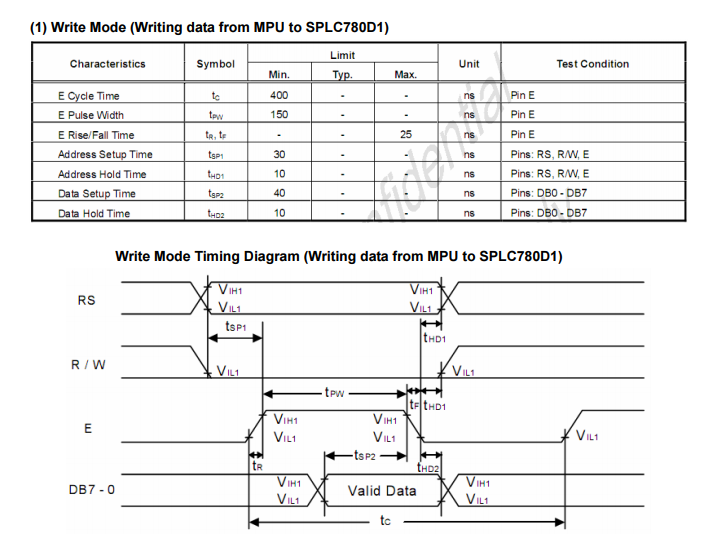
\includegraphics[width=\textwidth]{./img/1602_timing.png}
  \caption{LCD1602 Write AC Characteristic}\label{timing1602}
\end{figure}

根据要求,MCU应该做的步骤如下
\begin{enumerate}
\item 清零E线,初始化RS线(按需)和RW线(拉低)
\item 等待$t_sp1$(30ns),芯片设定写入状态
\item 拉高E线,使能芯片
\item 将数据线(8根)设定为需要的值
\item 等待$t_sp2$(40ns),等待写入完成
\item 拉低E线
\item 至少等待$t_hd1$(或$t_hd2$)(10ns),待数据建立后,可以再次使用RW、RS和DB线。
\end{enumerate}
在实际场景下,尤其是需要频繁更新数据时,应该严格按照手册时序进行,否则可能产生通信错
误。此外,两次拉高E的时间应不少于400ns。

本作业中,为了保证运行正常,将以上所有延时由ns扩至us级别。

\subsection{实现比较精确的延迟}

前几次作业中介绍了一种比较好用的定时方法:SysTick。利用这个定时器可以这么做。

首先,接管SysTick的处理函数。定义一个全局变量syscount,每次中断时,若该值不为0,则
将其减1,否则不做处理。

接着,配置systick,使其达到基本精确的1us延迟。

现在可以定义函数\lstinline{delay_10us},如下代码\ref{dly10us}
\begin{lstlisting}[caption={Use SYSTICK to delay},label={dly10us}]
void delay_10us(int i){
	i*=10;
	systicker=i;
	while(systicker);
}
\end{lstlisting}

这样,就用比较简单的方法实现了延迟。还有其他实现的方法,这里就不再介绍了。

\subsection{1602操作方法}

1602系列芯片的操作方法比较简单。上电后,首先复位控制器,选择好屏幕类型,接下来向特定的
内存地址写入即可。这里分析对地址和数据进行写入的方法,如清单\ref{lcd1602wr}。
\begin{lstlisting}[caption={LCD1602 write and read},label={lcd1602wr}]
void _lcd1602_write_data(unsigned short int  data){
	_LCD1602_UNSET_EN;
	_LCD1602_SET_RS;
	_LCD1602_UNSET_RW;
	//delay for 40us here
	delay_10us(4);
	//send command data
	LCD1602_WRITE_DATABAND( data );
	_LCD1602_SET_EN;
	//delay for at least 150ms here
	delay_10us(20);
	//stop process
	_LCD1602_UNSET_EN;
}

void _lcd1602_write_cmd(unsigned short int  data){
	_LCD1602_UNSET_EN;
	_LCD1602_UNSET_RS;
	_LCD1602_UNSET_RW;
	//delay for 40us here
	delay_10us(4);
	//send command data
	LCD1602_WRITE_DATABAND( data );
	_LCD1602_SET_EN;
	//delay for at least 150ms here
	delay_10us(20);
	//stop process
	_LCD1602_UNSET_EN;
}


void lcd1602_initalize(void){
	SysTick_Config(SystemCoreClock/100000);
	//Initalize related GPIO Ports
	GPIOInitalize();
	//screen reset
	_lcd1602_write_cmd( _LCD1602_CON_8BIT | _LCD1602_CON_2L | _LCD1602_CON_507 );	
	//cls if need
	#ifdef LCD1602_INIT_CLS
	lcd1602_cls();
	#endif
	//init default settings
	lcd1602_set_options(LCD1602_INIT_OPTIONS);	
}
\end{lstlisting}

\section{程序运行和分析}

运行之后显示的字符如\ref{lcdrun}所示。
\begin{figure}[h]
  \centering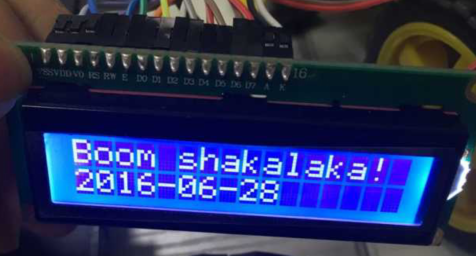
\includegraphics[width=\textwidth]{./img/1602_test.png}
  \caption{LCD1602 Test}\label{lcdrun}
\end{figure}

程序主文件如后附的各清单所示。代码较多,分为多个文件,因此分片进行大致讲解。

LCD1602开头的三个文件,也就是清单\ref{lcd1602ch}、\ref{lcd1602dh}、
\ref{lcd1602dc}是显示屏驱动的几个核心文件。后两个是驱动文件,定义了驱动函数,
并提供了几个外部接口函数,可直接打印字符串等。前一个为配置文件,其中不仅有简单
的对引脚的宏定义,还包含由一部分需要用宏来实现的位操作。以便应对数据线不连续
等情况。

heartrun\_mon开头的三个文件,也就是清单\ref{heartmonch}、\ref{heartmondh}、
\ref{heartmondc}是CPU状态监测灯的驱动文件,其作用与前几个类似。同样,以
serial\_debugger开头的三个文件,也就是清单\ref{serialdbgch}、\ref{serialdbgdh}、
\ref{serialdbgdc}是串口通信库,可以参见上一个报告中的有关介绍。

主程序如\ref{main}所示。

\begin{lstlisting}[caption={Main.c},label={main}]
#include "stm32f10x.h"
#include "lcd1602_driver.h"
#include "serial_debugger.h"
#include "heartrun_mon.h"

int main(void){
	unsigned int i = 0;
	//Initalize On-chip Periphals
	serialdbg_init();
	heartrun_mon_init();
	//wait for battery
	for ( i = 0 ; i < 0xffff; i++);
	lcd1602_initalize();
	
	serialdbg_printstr("\n\n");
	serialdbg_printstr("This is a serial commander!\n");
	serialdbg_printstr("Type and I'll tell you what you've typed!\n\n");
	
	lcd1602_putstring("Boom shakalaka!\n2016-06-28");
	
	while(1);

}
\end{lstlisting}

\begin{lstlisting}[caption={File serial\_debugger\_config.h},label={serialdbgch}]
#ifndef __SERIALDBG_CFG_H__
#define __SERIALDBG_CFG_H__

#define UsartTxPort GPIO_Pin_9
#define UsartRxPort GPIO_Pin_10
#define UsartGroup GPIOA
#define UsartGPIOClock RCC_APB2Periph_GPIOA
#define UsartClock RCC_APB2Periph_USART1

#ifdef SEPERATE_LED_USART
#define LEDTxPort GPIO_Pin_7
#define LEDRxPort GPIO_Pin_8
#define LEDGroup GPIOB
#define LEDGPIOClock RCC_APB2Periph_GPIOB
#endif
#endif
\end{lstlisting}

\begin{lstlisting}[caption={File serial\_debugger.h},label={serialdbgdh}]
#ifndef __SERIALDBG_DRV_H__
#define __SERIALDBG_DRV_H__

#include "stm32f10x.h"
#include "serial_debugger_config.h"

#ifdef SEPERATE_LED_USART
#define USART1_SENDOUT(data) do{USART_SendData(USART1,data);\
					blink(LEDGroup, LEDTxPort);\
					while(USART_GetFlagStatus(USART1, USART_FLAG_TC) == RESET);}while(0);
#else
#define USART1_SENDOUT(data) do{USART_SendData(USART1,data);\
					while(USART_GetFlagStatus(USART1, USART_FLAG_TC) == RESET);}while(0);
#endif

#define USART1_SENDCRLF() do{					USART_SendData(USART1,'\r');\
					while(USART_GetFlagStatus(USART1, USART_FLAG_TC) == RESET);\
					USART_SendData(USART1,'\n');}while(0);
void serialdbg_printstr(char* str);
void serialdbg_init(void);

#endif
\end{lstlisting}

\begin{lstlisting}[caption={File serial\_debugger.c},label={serialdbgdc}]
#include "serial_debugger.h"

#define blink(group, pin)   do{if (GPIO_ReadOutputDataBit((group), (pin))) \
							GPIO_ResetBits((group), (pin)); \
							else GPIO_SetBits((group), (pin));}\
							while(0);

void serialdbg_printstr(char* str){
	while(*str!='\0'){
		if (*str == '\n')
			USART1_SENDOUT('\r');
		USART1_SENDOUT(*str++);
	}
}


void USART1_IRQHandler(void){
	unsigned char x;
	if (USART_GetITStatus(USART1, USART_IT_RXNE)==SET){
		/* Received a byte */
		#ifdef SEPERATE_LED_USART
		blink(LEDGroup, LEDRxPort);
		#endif
		x=USART_ReceiveData(USART1);	//RXNE will be hw-cls by reading data
		while(USART_GetFlagStatus(USART1, USART_FLAG_TC) == RESET);	//wait till idle
		if (USART_GetITStatus(USART1, USART_IT_TXE)==RESET)	//make sure sendable
		switch (x) {
				case '\r'://make special process for CRLF
					USART1_SENDCRLF();
					break;
				case 0x7F:
				USART1_SENDOUT(8);
				USART1_SENDOUT(' ');
				USART1_SENDOUT(8);
					break;
				default:
				#ifdef ISDBG
					USART1_SENDOUT('*');
					USART1_SENDOUT(x);
					USART1_SENDOUT('=');
					USART_SendData(USART1, x);//send data back
					x=(x>>4)|(x<<4);
					USART1_SENDOUT((x&0xf)>10?(x&0xf)-10+'A':(x&0xf)+'0');//send data back
					x>>=4;
					USART1_SENDOUT((x&0xf)>10?(x&0xf)-10+'A':(x&0xf)+'0');//send data back
					USART1_SENDOUT('*');
				#else
					USART1_SENDOUT(x);
				#endif
		}
	}
}

void UsartInitalize(void){

	USART_InitTypeDef usart_initval;
	GPIO_InitTypeDef gpio_initval;
	RCC_APB2PeriphClockCmd(UsartGPIOClock, ENABLE);

	gpio_initval.GPIO_Speed = GPIO_Speed_50MHz;
	/* Tx port set*/
	gpio_initval.GPIO_Pin = UsartTxPort;
	gpio_initval.GPIO_Mode = GPIO_Mode_AF_PP;	//Need stronger output
	GPIO_Init(UsartGroup, &gpio_initval);
	/* Rx port set*/
	gpio_initval.GPIO_Pin = UsartRxPort;
	gpio_initval.GPIO_Mode = GPIO_Mode_IN_FLOATING;	//Need weeker input
	GPIO_Init(UsartGroup, &gpio_initval);
	
	/* Clock Initalize*/
	RCC_APB2PeriphClockCmd(UsartClock, ENABLE);		
	/* Configurements of USART1 */
	usart_initval.USART_BaudRate = 9600;									//baudrate is 600. notice sysclock
	usart_initval.USART_HardwareFlowControl 
					= USART_HardwareFlowControl_None ;						//no flow control
	usart_initval.USART_StopBits = USART_StopBits_1;			//1s
	usart_initval.USART_WordLength = USART_WordLength_8b;	//8d
	usart_initval.USART_Parity = USART_Parity_No;					//No check
	usart_initval.USART_Mode = 
						USART_Mode_Rx | USART_Mode_Tx;							//Do both job
	/* Write configure */
	USART_Init(USART1, &usart_initval);
	/* USART1 IRQn Triggerable */
	USART_ITConfig(USART1, USART_IT_RXNE, ENABLE);
	/* USART1 Bootup */
	USART_Cmd(USART1, ENABLE);
	/* USART1 IRQn NVIC Interruptable */
	NVIC_EnableIRQ(USART1_IRQn);
}

void serialdbg_init(void){
	UsartInitalize();
}
\end{lstlisting}


\begin{lstlisting}[caption={File heartrun\_mon\_cfg.h},label={heartmonch}]
#ifndef __HEARTRUNMON_CFG_H__
#define __HEARTRUNMON_CFG_H__

#define LEDRunPort GPIO_Pin_15
#define LEDGroup GPIOG
#define LEDGPIOClock RCC_APB2Periph_GPIOG

#endif
\end{lstlisting}

\begin{lstlisting}[caption={File heartrun\_mon.h},label={heartmondh}]
#ifndef __HEARTRUNMON_DRV_H__
#define __HEARTRUNMON_DRV_H__

#include "heartrun_mon_cfg.h"

void heartrun_mon_init(void);

#endif
\end{lstlisting}

\begin{lstlisting}[caption={File heartrun\_mon.c},label={heartmondc}]
#include "heartrun_mon.h"
#include "stm32f10x.h"


#define blink(group, pin)   do{if (GPIO_ReadOutputDataBit((group), (pin))) \
							GPIO_ResetBits((group), (pin)); \
							else GPIO_SetBits((group), (pin));}\
							while(0);

void GpioInitalize(void){
	GPIO_InitTypeDef gpio_initval;

	/* Open clock */
	RCC_APB2PeriphClockCmd(LEDGPIOClock, ENABLE);
	gpio_initval.GPIO_Speed = GPIO_Speed_50MHz;
	gpio_initval.GPIO_Pin = LEDRunPort;	//heartbeat led
	gpio_initval.GPIO_Mode = GPIO_Mode_Out_PP;
	GPIO_Init(LEDGroup, &gpio_initval);
}

void TimerInitalize(void){

	TIM_TimeBaseInitTypeDef tim_tb_initval;

	//Enable timer of heart beat
	RCC_APB1PeriphClockCmd(RCC_APB1Periph_TIM2, ENABLE);  
	TIM_DeInit(TIM2);	 //Reset to default
	/* Set timer to 4Hz */
	tim_tb_initval.TIM_Prescaler = 36000; 
	tim_tb_initval.TIM_ClockDivision = TIM_CKD_DIV1;	
	tim_tb_initval.TIM_CounterMode = TIM_CounterMode_Up;	
	tim_tb_initval.TIM_Period =  300-1;//0.15s	  	
	TIM_TimeBaseInit(TIM2, &tim_tb_initval);	//apply settings
	TIM_ClearFlag(TIM2, TIM_FLAG_Update);		//clear flag
	TIM_ITConfig(TIM2, TIM_IT_Update, ENABLE);	//can set interruption
	TIM_Cmd(TIM2, ENABLE);		//enable Timer2
	NVIC_EnableIRQ(TIM2_IRQn);	//Enable IRQ in NVIC

}

void heartrun_mon_init(void){
	GpioInitalize();
	TimerInitalize();
}

void TIM2_IRQHandler(void){
	if (TIM_GetITStatus(TIM2, TIM_IT_Update)!=RESET){
		TIM_ClearITPendingBit(TIM2, TIM_FLAG_Update);	//Clear IT Flag
		blink(LEDGroup, LEDRunPort);	//Show the heartbeat
	}
}
\end{lstlisting}

\begin{lstlisting}[caption={File lcd1602\_config.h},label={lcd1602ch}]
#ifndef __LCD1602_CFG_H__
#define __LCD1602_CFG_H__

#define LCD1602_RS 		 GPIO_Pin_13
#define LCD1602_RW 		 GPIO_Pin_14
#define LCD1602_E  		 GPIO_Pin_15

#define LCD1602_RS_GROUP GPIOC
#define LCD1602_RW_GROUP GPIOC
#define LCD1602_E_GROUP  GPIOC

#define LCD1602_RS_CLOCK RCC_APB2Periph_GPIOC
#define LCD1602_RW_CLOCK RCC_APB2Periph_GPIOC
#define LCD1602_E_CLOCK  RCC_APB2Periph_GPIOC

#define LCD1602_CLOCK_Cmd(X,Y) RCC_APB2PeriphClockCmd((X),(Y))

//We need to use macro to deal with different type of value read/write to increase speed
//In this example our data is from E7->E14
//which means to read it, just read group E and have E>>7
#define LCD1602_WRITE_DATABAND(data) do{ GPIOF->BSRR = ((data&0xff) | ((~data)&0xff)<<(+16)) ;}while(0);
#define LCD1602_READ_DATABAND 		(((GPIOF->IDR))&0xff)

//Follow options define initalize behaviour
#define LCD1602_CAN_SCREENMOVE
#define LCD1602_INIT_CLS
#define LCD1602_LINE_COUNT 2
#define LCD1602_CHAR_COUNT 16
#define LCD1602_INIT_OPTIONS ( LCD1602_CURSOR_AUTORIGHT | LCD1602_DISP_ON | LCD1602_CURSOR_OFF | LCD1602_CURSOR_STILL )

#endif
\end{lstlisting}
\begin{lstlisting}[caption={File lcd1602\_driver.h},label={lcd1602dh}]
#ifndef __LCD1602_DRV_H__
#define __LCD1602_DRV_H__

#include "lcd1602_config.h"

/* Cursor movement commands */
#define LCD1602_CURSOR_LEFT 0x10
#define LCD1602_CURSOR_RIGHT 0x14

//Followings are used only if your screen support move
#ifdef LCD1602_CAN_SCREENMOVE
#define LCD1602_SCREEN_LEFT 0x18
#define LCD1602_SCREEN_RIGHT 0x1C
#define LCD1602_SCREEN_NOAUTOMOV (0x4<<__LCD1602_CURSOR_CFG_OFFSET)
#define LCD1602_SCREEN_AUTORIGHT  (0x5<<__LCD1602_CURSOR_CFG_OFFSET)
#endif

/* Those configure values should be bitor*/
// Cursor/Screen mov config
#define LCD1602_CURSOR_AUTOLEFT   (0x4<<__LCD1602_CURSOR_CFG_OFFSET)
#define LCD1602_CURSOR_AUTORIGHT  (0x6<<__LCD1602_CURSOR_CFG_OFFSET)
#define __LCD1602_CURSOR_CFG_OFFSET 0
#define _LCD1602_GET_CURSOR_CONFIG(config) (((config)>>__LCD1602_CURSOR_CFG_OFFSET)&0x7)
// Display Config
#define LCD1602_DISP_OFF     (0x8<<__LCD1602_DISP_CFG_OFFSET)
#define LCD1602_DISP_ON      (0xC<<__LCD1602_DISP_CFG_OFFSET)
#define LCD1602_CURSOR_OFF   (0x8<<__LCD1602_DISP_CFG_OFFSET)
#define LCD1602_CURSOR_ON    (0xA<<__LCD1602_DISP_CFG_OFFSET)
#define LCD1602_CURSOR_STILL (0x8<<__LCD1602_DISP_CFG_OFFSET)
#define LCD1602_CURSOR_BLINK (0x9<<__LCD1602_DISP_CFG_OFFSET)
#define __LCD1602_DISP_CFG_OFFSET 3
#define _LCD1602_GET_DISP_CONFIG(config) (((config)>>__LCD1602_DISP_CFG_OFFSET)&0xF)

/* Controller Configs which will not merged with others */
#define _LCD1602_CON_4BIT		 0x20
#define _LCD1602_CON_8BIT		 0x30
#define _LCD1602_CON_1L			 0x20
#define _LCD1602_CON_2L			 0x28
#define _LCD1602_CON_507		 0x20
#define _LCD1602_CON_510		 0x24

/* Macros used to operate function lines */
//chip set=enable unset=disable
#define _LCD1602_SET_EN GPIO_SetBits(LCD1602_E_GROUP, LCD1602_E);
#define _LCD1602_UNSET_EN GPIO_ResetBits(LCD1602_E_GROUP, LCD1602_E);
//chip set=read unset=write
#define _LCD1602_SET_RW GPIO_SetBits(LCD1602_RW_GROUP, LCD1602_RW);
#define _LCD1602_UNSET_RW GPIO_ResetBits(LCD1602_RW_GROUP, LCD1602_RW);
//chip set=data unset=command
#define _LCD1602_SET_RS GPIO_SetBits(LCD1602_RW_GROUP, LCD1602_RS);
#define _LCD1602_UNSET_RS GPIO_ResetBits(LCD1602_RW_GROUP, LCD1602_RS);

/* Some fixed value of command */
#define _LCD1602_CLS 0x1
#define _LCD1602_CR 0x2

/* Macros */
//convert value to CGRAM or DDRAM address
#define _LCD1602_ADDR_CGRAM(data) (((data)&0x3F)|0x40)
#define _LCD1602_ADDR_DDRAM(data) (((data)&0x7F)|0x80)
//abstract value from read value
#define _LCD1602_CONVERT_BUSY(data) ((data)&0x80)
#define _LCD1602_CONVERT_ACPOS(data) ((data)&0x7F)

//Initalization
void lcd1602_initalize(void);

//Clean the screen
void lcd1602_cls(void);

//Carrage return to left
void lcd1602_cr(void);

//Set config value with LCD1602_CFG values
void lcd1602_set_options(unsigned int config_value);

//put a char
void lcd1602_putchar(char ch);

//put a string
void lcd1602_putstring(char str[]);

//use macro define to do cursor move
void lcd1602_cursor_move(unsigned int move);


#endif
\end{lstlisting}
\begin{lstlisting}[caption={File lcd1602\_driver.c},label={lcd1602dc}]
#include "lcd1602_driver.h"
#include "stm32f10x.h"

unsigned int systicker = 0;

void delay_10us(int i){
	i*=10;
	systicker=i;
	while(systicker);
}

void SysTick_Handler(void){
	if (systicker!=0)
		systicker--;
}

void GPIOInitalize(void){
	GPIO_InitTypeDef gpio_initval;
	//Command port initalize
	RCC_APB2PeriphClockCmd(RCC_APB2Periph_GPIOC, ENABLE);
	gpio_initval.GPIO_Mode = GPIO_Mode_Out_PP;
	gpio_initval.GPIO_Speed = GPIO_Speed_50MHz;
	gpio_initval.GPIO_Pin = LCD1602_RS;
	GPIO_Init(LCD1602_RS_GROUP, &gpio_initval);
	gpio_initval.GPIO_Pin = LCD1602_RW;
	GPIO_Init(LCD1602_RW_GROUP, &gpio_initval);
	gpio_initval.GPIO_Pin = LCD1602_E;
	GPIO_Init(LCD1602_E_GROUP, &gpio_initval);

	//Data port
	//#error Be sure you have initalized related DATA pins before you remove this line of error message!!!
	RCC_APB2PeriphClockCmd(RCC_APB2Periph_GPIOF, ENABLE);
	gpio_initval.GPIO_Pin = GPIO_Pin_All;
	GPIO_Init(GPIOF,&gpio_initval);
}

void _lcd1602_write_data(unsigned short int  data){
	_LCD1602_UNSET_EN;
	_LCD1602_SET_RS;
	_LCD1602_UNSET_RW;
	//delay for 40us here
	delay_10us(4);
	//send command data
	LCD1602_WRITE_DATABAND( data );
	_LCD1602_SET_EN;
	//delay for at least 150ms here
	delay_10us(20);
	//stop process
	_LCD1602_UNSET_EN;
}

void _lcd1602_write_cmd(unsigned short int  data){
	_LCD1602_UNSET_EN;
	_LCD1602_UNSET_RS;
	_LCD1602_UNSET_RW;
	//delay for 40us here
	delay_10us(4);
	//send command data
	LCD1602_WRITE_DATABAND( data );
	_LCD1602_SET_EN;
	//delay for at least 150ms here
	delay_10us(20);
	//stop process
	_LCD1602_UNSET_EN;
}


void lcd1602_initalize(void){
	SysTick_Config(SystemCoreClock/100000);
	//Initalize related GPIO Ports
	GPIOInitalize();
	//screen reset
	_lcd1602_write_cmd( _LCD1602_CON_8BIT | _LCD1602_CON_2L | _LCD1602_CON_507 );	
	//cls if need
	#ifdef LCD1602_INIT_CLS
	lcd1602_cls();
	#endif
	//init default settings
	lcd1602_set_options(LCD1602_INIT_OPTIONS);	
}

void lcd1602_cls(void){	
	_lcd1602_write_cmd(_LCD1602_CLS);
}

void lcd1602_cursor_move(unsigned int move){	
	_lcd1602_write_cmd(move);
}

void lcd1602_cursor_pos(unsigned short int line, unsigned short int pos){
	_lcd1602_write_cmd( _LCD1602_ADDR_DDRAM( 
			(line<LCD1602_LINE_COUNT?line<<6:(line%LCD1602_LINE_COUNT)<<6) + 
			(pos<LCD1602_CHAR_COUNT?pos:pos%LCD1602_CHAR_COUNT) ));
}

void lcd1602_cr(void){
	_lcd1602_write_cmd(_LCD1602_CR);
}

void lcd1602_set_options(unsigned int config_value){
	if (_LCD1602_GET_CURSOR_CONFIG(config_value))
		_lcd1602_write_cmd(_LCD1602_GET_CURSOR_CONFIG(config_value));
	if (_LCD1602_GET_DISP_CONFIG(config_value)){
		delay_10us(20);//wait till still
		_lcd1602_write_cmd(_LCD1602_GET_DISP_CONFIG(config_value));
	}
}

void lcd1602_putchar(char ch){
	_lcd1602_write_data(ch);
}

void lcd1602_putstring(char str[]){
	char* cur = str;
	while(cur - str < 0x20 && *cur!='\0'){
		if ( cur - str == LCD1602_CHAR_COUNT)
			lcd1602_cursor_pos(1,0);
		if (*cur=='\n'){
			lcd1602_cursor_pos(1,0);
			cur++;
		}
		else
			lcd1602_putchar(*cur++);
	}
}
\end{lstlisting}

\end{document}
